\documentclass{beamer}
\usetheme{default}


\title{ECE411 Final Presentation}
\subtitle{Womprats T-16 Audio Synthesizer}
\author{A. Goetz \and B. Kanyid \and J. Pugh \and K. Riedl}
\institute[PSU]{
  Maseeh College of Engineering and Computer Science\\
  Portland State University\\
  Portland, Oregon 97207  
}
\date{\today}


\begin{document}
\begin{frame}[plain]
  \titlepage
\end{frame}


%\frame{\titlepage}
\frame{\frametitle{Agenda}\tableofcontents} 


% 30 seconds for overview
\section{Project Overview} 
\frame{\frametitle{Project Overview} 
[Overview text here]
Audio synthesizers provide entertainment by creating unique sounds.
}
\subsection{Objective}
\frame{{Objective}
[Objective text here]
Design and build a device that can generate sounds from user-control.
}
\subsection{Requirements}
\frame{{Requirements}
[Requirements text here]

}
\subsection{Approach}
\frame{{Approach}
[Approach text here]
Project management/documentation tools: Gantt chart, redmine/wiki\\
Technical tools: kicad, lpcexpresso/redcode
}

\section{Design}
\frame{\frametitle{Design}
[Design text here]
}
\subsection{Implementation}
\frame{{Implementation}
[Implementation text here]
}

\subsection{PCB Layout}
\frame{{PCB Layout} 
\begin{center}
 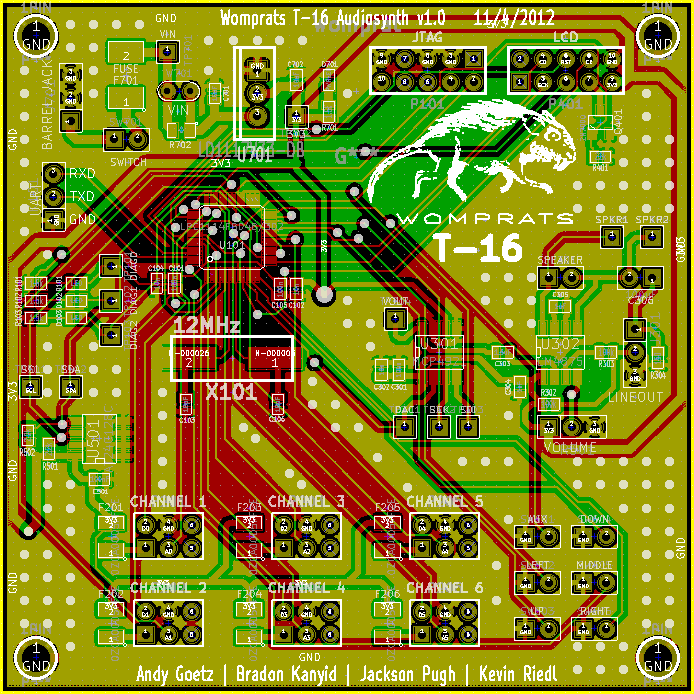
\includegraphics[width=0.7\textwidth]{pcb.png} 
\end{center}
}

\subsection{Testing \& Debugging}
\frame{{Testing \& Debugging}
[Testing \& Debugging text here]

}
\subsection{Results}
\frame{{Results}
[Results text here]
}

\section{Team Evaluation}
\frame{\frametitle{Team Evaluation}
[Team Evaluation text here]
}
\subsection{Contributions}
\frame{{Contributions}
[Contributions text here]
}
\subsection{Lessons Learned}
\frame{{Lessons Learned}
[Lessons Learned text here]
}


%\section{Design Choices}
%\frame{\frametitle{Design Choices} 
%Design Choices text here
%}

%\begin{frame}{Design Choices}
%  \begin{itemize}
%    \pause
%  \item KiCad
%    \pause
%  \item LPC1114
%    \pause
%  \item GanttProject
%    \pause
%  \item \LaTeX
%    \end{itemize}
%\end{frame}



\end{document}
